% $Id: macros.tex,v 1.8 2012/07/19 22:21:36 ccamacho Exp $
% \newenvironment{definition}{\par\bf\bigskip \bigskip Definition}{\bigskip \bigskip}{\rmfamily}
% \newenvironment{example}{\par\bf\bigskip \bigskip Example}{\bigskip \bigskip}{\rmfamily}
% \newenvironment{lemma}{\par\bf\bigskip \bigskip  Lemma}{\bigskip \bigskip}{\rmfamily}
% \newenvironment{proof}{\par{\bf\bigskip \bigskip  Proof}}{\bigskip \bigskip}{\rmfamily}
% \newenvironment{proposition}{\par\bf \bigskip\bigskip  Proposition}{\bigskip \bigskip}{\rmfamily}
% \newenvironment{corollary}{\par\bf \bigskip\bigskip  Corollary}{\bigskip \bigskip}{\rmfamily}
% \newenvironment{theorem}{\par\bf \bigskip \bigskip Theorem}{\bigskip \bigskip}{\rmfamily}

%Fin de Carlos

% $Id: macros.tex,v 1.8 2012/07/19 22:21:36 ccamacho Exp $
\def\squareforqed{\hbox{\rlap{$\sqcap$}$\sqcup$}}

% Carlos
% He eliminado los cubos del qed, luego podemos mirar
% si queda algun simbolo mejor
\def\qed{
       \ifmmode\squareforqed\else{\unskip\nobreak\hfil
    \penalty50\hskip1em\null\nobreak\hfil\squareforqed
    \parfillskip=0pt\finalhyphendemerits=0\endgraf}\fi
}

%\usepackage{marginnote}
%\renewcommand{\marginfont}{\fontsize{6}{8}\selectfont}



\newcommand{\ccomens}[2]{\uwave{#1\ccomen{#2}}}
\def\lcomen#1{\footnote{\textbf{Comentario de Luis}: \textcolor{red}{#1}}}
\def\ccomen#1{\footnote{\textbf{Comentario de Carlos}: \textcolor{blue}{#1}}}
\def\acomen#1{\footnote{\textbf{Comentario de Alberto}: \textcolor{green}{#1}}}



\newcommand{\comment}[2]{\footnote{\textbf{#1}: #2}}

\newcommand{\ComaMat}{}
\newcommand{\PuntoMat}{}
%\newenvironment{proof}{Proof}


\newcommand{\ismcomment}[1]{}
\newcommand{\bdfn}{\begin{definition} \begin{rm}}
\newcommand{\edfn}{\end{rm}$ $\qed \end{definition}}

\newcommand{\bprf}{\begin{proof}}
\newcommand{\eprf}{\leavevmode\qed \end{proof}}

\newcommand{\bthm}{\begin{theorem} \begin{rm}}
\newcommand{\ethm}{\end{rm}$ $\qed \end{theorem}}

\newcommand{\bprop}{\begin{proposition} \begin{rm}}
\newcommand{\eprop}{\end{rm}$ $\qed  \end{proposition}}

\newcommand{\bcor}{\begin{corollary}\begin{rm}}
\newcommand{\ecor}{\end{rm}$ $\qed  \end{corollary}}

\newcommand{\blem}{\begin{lemma}\begin{rm}}
\newcommand{\elem}{\end{rm}$ $\qed  \end{lemma}}

\newcommand{\bfact}{\begin{fact}\begin{rm}}
\newcommand{\efact}{\end{rm}$ $\qed  \end{fact}}

\newcommand{\bex}{\begin{example}\begin{rm}}
\newcommand{\eex}{\end{rm}$ $\qed  \end{example}}

\newenvironment{defn}{\bdfn}{\edfn}
\newenvironment{proofappendix}[1]{\textbf{\emph{Proof of #1}}}{}
\newcommand{\barra}{\:| \:}
\def\y{\;\wedge\;}
\def\o{\;\vee\;}
\newcommand{\union}{\cup}
\newcommand{\contenido}{\subseteq}
\newcommand{\interseccion}{\cap}
\newcommand{\Vacio}{\emptyset}
\renewcommand{\emptyset}{\varnothing}

\newcommand{\true}{\mathtt{true}}
\newcommand{\false}{\mathtt{false}}
\newcommand{\entonces}{\mathtt{\ then\  }}
\newcommand{\sino}{\mathtt{\ else\  }}
\newcommand{\si}{\ \mathrm{if}\ }

\newcommand{\letbar}[1]{\mbox{I\kern-0.23em#1}}
%\newcommand{\nat}{\letbar N}
%\newcommand{\real}{\letbar R}
\newcommand{\real}{\mathbb{R}}
\newcommand{\realm}{\letbar R_+^m}
\newcommand{\Bool}{\texttt{Bool}}
%
\newcommand{\comen}[1]{
}
\newcommand{\timed}{{\mathtt{Time}}}
\newcommand{\outputs}[1]{\ensuremath{\mathtt{ outputs}(#1)}}
\newcommand{\representative}[2]{\ensuremath{\mathtt{ moreR}(#1,#2)}}
\newcommand{\msTOs}[1]{\ensuremath{\mathtt{ msTOs}(#1)}}
\newcommand{\setnttr}[2]{\ensuremath{\mathtt{ setnttr}(#1,#2)}}
\newcommand{\minTime}[1]{\ensuremath{\mathtt{ mT}(#1)}}
\newcommand{\maxTime}[1]{\ensuremath{\mathtt{ MT}(#1)}}
\newcommand{\minimo}[1]{\ensuremath{\mathtt{ min}\left\{\!#1 \!\!\!\!\right\}}}
\newcommand{\maximo}[1]{\ensuremath{\mathtt{ max}\left\{\!#1 \!\!\!\!\right\}}}
\newcommand{\FSM}{\texttt{FSM}}
\newcommand{\FSMs}{\texttt{FSMs}}
\newcommand{\EFSM}{\texttt{EFSM}}
\newcommand{\EFSMs}{\texttt{EFSMs}}
\newcommand{\TFSM}{\texttt{TFSM}}
\newcommand{\TFSMs}{\texttt{TFSMs}}
\newcommand{\TPEM}{\texttt{TPEM}}
\newcommand{\TPEMs}{\texttt{TPEMs}}

\newcommand{\SPLs}{\texttt{SPLs}}
\newcommand{\SPL}{\texttt{SPL}}
\newcommand{\PLs}{\texttt{PLs}}
\newcommand{\PL}{\texttt{PL}}
\newcommand{\FODAT}{\texttt{AT}}

\newcommand{\FODA}{\texttt{FODA}}
\newcommand{\fodaPA}{\ensuremath{\mathtt{SPLA}}}
\newcommand{\fodaPAc}{\ensuremath{\mathtt{SPLA{^\calC}}}}
\newcommand{\fodaPAp}{\ensuremath{\mathtt{SPLA{^\calP}}}}
\newcommand{\fodaPAbasic}{\ensuremath{\mathtt{fodaA_b}}}
\newcommand{\wellstructured}{\ensuremath{\mathtt{fodaA_{ws}}}}
\newcommand{\normalForm}{\ensuremath{\mathtt{fodaA_{nf}}}}
\newcommand{\prenormalForm}{\ensuremath{\mathtt{fodaA_{pre}}}}
\newcommand{\RSEB}{\texttt{RSEB}}
\newcommand{\PLUSS}{\texttt{PLUSS}}
\newcommand{\np}{\mathtt{np}}




 %

\newcommand{\afterCond}[1]{\texttt{afterCond}(#1)}
\newcommand{\afterInp}[1]{\texttt{afterInp}(#1)}
\newcommand{\IUT}{\texttt{IUT}}
%\newcommand{\case}{\texttt{Case :}}
\newcommand{\HOTL}{{\cal HOTL}}
\newcommand{\wc}{wild-card}

\newcommand{\calA}{{\cal A}}
\newcommand{\calB}{{\cal B}}
\newcommand{\calC}{{\cal C}}
\newcommand{\calD}{{\cal D}}
\newcommand{\calE}{{\cal E}}
\newcommand{\calF}{{\cal F}}
\newcommand{\calG}{{\cal G}}
\newcommand{\calH}{{\cal H}}
\newcommand{\calI}{{\cal I}}
\newcommand{\calL}{{\cal L}}
\newcommand{\calM}{{\cal M}}
\newcommand{\calN}{{\cal N}}
\newcommand{\calO}{{\cal O}}
\newcommand{\calP}{{\cal P}}
\newcommand{\calQ}{{\cal Q}}
\newcommand{\calR}{{\cal R}}
\newcommand{\calS}{{\cal S}}
\newcommand{\calT}{{\cal T}}
\newcommand{\calU}{{\cal U}}
\newcommand{\calV}{{\cal V}}
\newbox\arriba
\newbox\abajo
\newbox\CaracterInterno
\newbox\CaracterDerecha
\newdimen\anchura
\def\MacrosTranGeneral#1#2#3#4#5#6{%
  \setbox\CaracterInterno=\hbox{\mathsurround=0pt$\mathord#4$}
  \setbox\CaracterDerecha=\hbox{\mathsurround=0pt$\mathord#3$}
  \setbox\arriba=\hbox{$#1#2$}
  \setbox\abajo=\hbox{\mathsurround=0pt%
                      \anchura=\wd\arriba%
                      \advance \anchura by 0.5em%
                      \divide \anchura by \wd\CaracterInterno%
                      \multiply \anchura by \wd\CaracterInterno%
                      \copy\CaracterInterno\kern\SeparacionInternaFlecha
                      \hbox to \anchura{%
                          $\cleaders%
                            \hbox{\kern\SeparacionInternaFlecha\copy\CaracterInterno}
                            \hfill$}%
                      \kern\SeparacionExternaFlecha\copy\CaracterDerecha}
  \mathrel{{\buildrel\vbox{\copy\arriba \kern\SeparacionFlechaArriba} %
    \over{\copy\abajo^{#6}}}_{#5}}
  }
\def\MacrosTranGeneralProp#1#2#3#4#5{\mathchoice%
  {\MacrosTranGeneral{\scriptstyle}{#1}{#2}{#3}{#4}{#5}}
  {\MacrosTranGeneral{\scriptstyle}{#1}{#2}{#3}{#4}{#5}}
  {\MacrosTranGeneral{\scriptscriptstyle}{#1}{#2}{#3}{#4}{#5}}
  {\MacrosTranGeneral{\scriptscriptstyle}{#1}{#2}{#3}{#4}{#5}}}

\def\MacrosTran#1{%
  \def\SeparacionInternaFlecha{-0.3em}
  \def\SeparacionExternaFlecha{-0.5em}
  \def\SeparacionFlechaArriba{-3pt}
  \MacrosTranGeneralProp{#1}{\rightarrow}{-}{}{}}
\def\MacrosNoTran#1{%
  \def\SeparacionInternaFlecha{-0.3em}
  \def\SeparacionExternaFlecha{-0.5em}
  \def\SeparacionFlechaArriba{-3pt}
  \MacrosTranGeneralProp{#1\kern 0.5em}{{\not\rightarrow}}{-}{}{}}
\def\MacrosVTran#1{%
  \def\SeparacionInternaFlecha{-0.2em}
  \def\SeparacionExternaFlecha{-0.5em}
  \def\SeparacionFlechaArriba{0pt}
  \MacrosTranGeneralProp{#1}{\Rightarrow}{=}{}{}}
\def\MacrosNoVTran#1{%
  \def\SeparacionInternaFlecha{-0.2em}
  \def\SeparacionExternaFlecha{-0.5em}
  \def\SeparacionFlechaArriba{-3pt}
  \MacrosNoTranGeneralProp{#1}{\not\Rightarrow}{=}{}{}}
\def\tran#1{\ensuremath\mathbin{\MacrosTran{#1}}}
\def\vtran#1{\ensuremath\mathbin{\MacrosVTran{#1}}}
\def\notran#1{\ensuremath\mathbin{\MacrosNoTran{#1}}}
\def\novtran#1{\ensuremath\mathbin{\MacrosNoVTran{#1}}}

\newcommand{\tranp}[2]{\MacrosTran{#1}_{\!\!#2}\;}
\newcommand{\tranap}[2]{\MacrosVTran{#1}_{\!\!#2}\;}
\newcommand{\tranb}[2]{\stackrel{#1}{\Longrightarrow}_{#2}}
\newcommand{\transi}[2]{\MacrosTran{#1}_{\!\!#2}\;}
\newcommand{\SSS}{\texttt{SSadmin}}
\newcommand{\calIR}{{\cal I\!R}}
\newcommand{\calDB}{{\cal D\!B}}

\newcommand{\vtranp}[2]{\vtran{#1}_{#2}}
\newcommand{\tranop}[2]{\MacrosNoTran{#1}_{\!\!#2}\;}


\newcommand{\product}[1]{\lfloor #1\rfloor}
\newcommand{\waste}{\ensuremath{\mathtt{waste}}}
\newcommand{\ham}{\ensuremath{\mathtt{TotProb}}}
\newcommand{\nombreRegla}[1]{\ensuremath{\mathbf{[#1]}}}
\newcommand{\tvacia}{\ensuremath{\epsilon}}
\newcommand{\traces}[1]{\ensuremath{\mathtt{tr}(#1)}}
\newcommand{\products}[1]{\ensuremath{\mathtt{prod}\left(#1\right)}}
\newcommand{\nttraces}[1]{\ensuremath{\mathtt{nttr}(#1)}}


\newcommand{\straces}[1]{\ensuremath{\mathtt{SuccessfulT}(#1)}}
\newcommand{\untraces}[1]{\ensuremath{\mathtt{UnsuccessfulT}(#1)}}
\renewcommand{\prod}{\ensuremath{\mathtt{prod}}}
\newcommand{\prodp}{\ensuremath{\mathtt{prod}^\calP}}
\newcommand{\prob}[1]{\ensuremath{\mathtt{prob}\left(#1\right)}}
\newcommand{\equivprob}{\ensuremath{\mathrel{\equiv^\calP}}}




\renewcommand{\prod}{\ensuremath{\mathtt{prod}}}
\newcommand{\values}{\ensuremath{\mathrm{Val}}}
\newcommand{\suminputs}[1]{\ensuremath{\mathtt{sumin}(#1)}}
\newcommand{\finish}[1]{\ensuremath{\mathtt{s}(#1)}}
\newcommand{\ptraces}[1]{\ensuremath{\mathtt{ptr}(#1)}}
\newcommand{\itraces}[1]{\ensuremath{\mathtt{itr}(#1)}}
\newcommand{\completeprob}[1]{\texttt{prob}(#1)}
\newcommand{\paral}{\ensuremath{\mathbin{\wedge}}}
\newcommand{\completion}[1]{\texttt{comp}(#1)}
\newcommand{\suma}[1]{\ensuremath{\mathtt{sum}(#1)}}
\newcommand{\ctraces}[1]{\ensuremath{\mathtt{CompleteT}(#1)}}




\newcommand{\testu}[1]{\ensuremath{\mathtt{tu}(#1)}}
\newcommand{\cover}[2]{\ensuremath{\mathtt{c}_{#1}(#2)}}
\newcommand{\generateTA}[1]{\texttt{generateT}(#1)}
\newcommand{\generateTB}[1]{\texttt{generateT'}(#1)}

\newcommand{\generateTAux}[1]{\texttt{generateTAux}(#1)}
%-----------------
% feature
\newcommand{\feature}[1]{\ensuremath{\mathtt{#1}}}
\newcommand{\f}[1]{\feature{#1}}
%Optional feature
\newcommand{\ofeature}[1]{\ensuremath{\overline{\feature{#1}}}}
\newcommand{\of}[1]{\ofeature{#1}}

%trace
\newcommand{\nil}{\ensuremath{\mathtt{nil}}}
\newcommand{\exclude}[3]{\feature{#1}\mathbin{\not\Rightarrow}\feature{#2}\ \mathtt{in}\ #3}
\newcommand{\require}[3]{\feature{#1}\mathbin{\Rightarrow}\feature{#2}\ \mathtt{in}\ #3}
\newcommand{\forbid}[2]{#2\backslash\feature{#1}}
\newcommand{\mandatory}[2]{#2\Rightarrow\feature{#1}}
\newcommand{\choice}{\mathbin{\lor}}
\newcommand{\optional}[1]{\overline{#1}}
\newcommand{\trace}[1]{\ensuremath{\langle #1 \rangle}}
\newcommand{\hide}[1]{[#1]}
\newcommand{\hideA}{\hide{\calA}}

\newcommand{\aviso}[1]{{\large\textbf{\texttt{Aviso:} #1}}.}


\newcommand{\refequation}[2]{\textbf{[#1\ref{#2}]}}
\newcounter{equationi}
\newenvironment{equations}[1]{%
  \begin{list}{\fequation{#1\arabic{equationi}}}{\usecounter{equationi}}
  \def\eqitem##1{\item\label{ax:#1##1}}
}{%
  \end{list}
}
\def\sizeeq{\fontsize{8}{7}\selectfont}
\def\fequation#1{\textbf{[#1]}}
\def\refequation#1#2{\fequation{#1\ref{ax:#1#2}}}
\def\fequationas#1{\quad{\fontsize{6}{8}\selectfont\fequation{#1}}}
\def\refequationas#1#2{\quad{\fontsize{6}{8}\selectfont\refequation{#1}{#2}}}
\usepackage{tikz}
%\usepackage{tikz-uml}
\usetikzlibrary{trees,shapes,arrows,automata,positioning}
\tikzset{
            syntax/.style={
                   rectangle,
                   rounded corners,
                   draw=black, very thick,
                   minimum height=2em,
                   inner sep=2pt,
                   text centered,
                   },
            feature/.style={
             rectangle,draw
            },
            triangle/.style = {
              regular polygon,regular polygon sides=3,draw
            },
            tree/.style={
              isosceles triangle, scale=0.7, shape border rotate=90, draw
            }
        }

\def\specification{
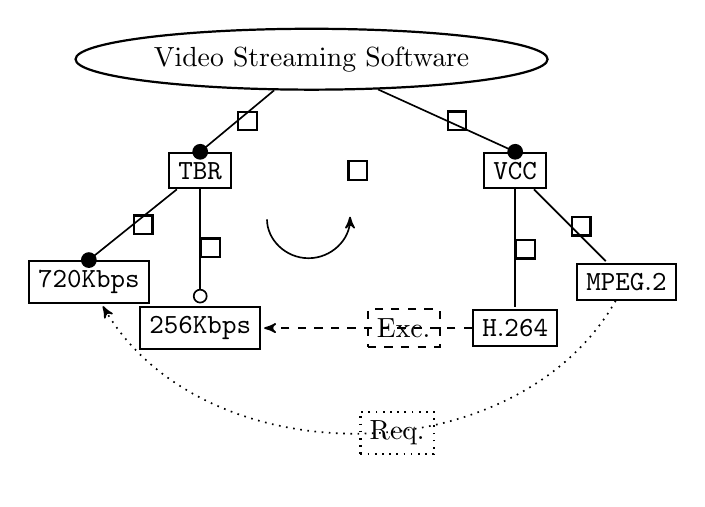
\begin{tikzpicture}[>=stealth',shorten >=1pt,auto,node distance=2cm, semithick,edge from parent]
  \node[ellipse,draw] (A)   {Video Streaming Software};
  \node[rectangle,draw]    (B) [below left  of=A]   {\TXBITRATE};
  \node[]    (AUX) [right  of=B]   {};
  \node[rectangle,draw]    (C) [right   of=AUX]   {\VCC};
  \node[rectangle,draw]    (D) [below left   of=B]   {\STZKPS};
  \node[rectangle,draw]    (E) [below of=B]   {\TFSKPS};
  \node[rectangle,draw]    (F) [below of=C]   {\HTSF};
  \node[rectangle,draw]    (G) [below right of=C]   {\MPEGTWO};

  \path (A) edge [] node {} (B.north)

            edge [] node {} (C.north)

        (B) edge [] node {} (D.north)
            edge [-o, fill] node {} (E)

        (C) edge [] node {} (F)

            edge []  node {} (G)

        (F) edge [->,dashed]  node {Exc.} (E)

        (G) edge [->,dotted,bend left=60]  node {Req.} (D)

  ;

\fill (B.north) circle (-0.1);
\fill (C.north) circle (-0.1);
\fill (D.north) circle (-0.1);
%\fill (-1.3,-1.3) circle (0.1);
%\fill (2.4,-1.3) circle (0.1);
%\fill (-3,-3) circle (0.1);

\draw [<-] (3.5,-2)  arc (360:180:15pt);

%\draw [fill=black](0,-0.35) -- (-0,-0.6) -- (0.6,-0.6)-- (0.35,-0.35)--(0,-0.35);

%\draw [<-] (A.south east)  arc (360:180:14pt);



%\draw [<-] (0.5,-0.2)  arc (360:180:14pt);

%\draw [<-] (-1.1,-4.2)  arc (360:180:14pt);

%\draw [<-] (1.5,-4.2)  arc (360:180:14pt);

%\draw [fill=black](-0.25,-4.85) -- (-0.5,-5.1) -- (0.2,-5.1)-- (0.1,-4.85)--(-0.25,-4.85);

%\draw [fill=black](2.4,-4.85) -- (2.5,-5.1) -- (3.20,-5.1)-- (2.75,-4.85)--(2.35,-4.85);

\end{tikzpicture}
}


\newcommand{\semden}[1]{\ensuremath{[\![#1]\!]}}
\newcommand{\Semden}[1]{\ensuremath{\left[\!\!\left[#1\right]\!\!\right]}}
\newcommand{\semdenp}[1]{\ensuremath{[\![#1]\!]^\calP}}
\newcommand{\Semdenp}[1]{\ensuremath{\left[\!\!\left[#1\right]\!\!\right]^\calP}}
\newcommand{\accum}{\mathtt{accum}}
\newcommand{\menos}{\mathbin{\backslash}}
\newcommand{\op}{\ensuremath{\mathtt{op}}}
\newcommand{\igecu}{\mathbin{=_{E}}}
\newcommand{\vocabulary}[1]{\ensuremath{\mathsf{voc}(#1)}}
\def\spaceFigure{0.3em}
\def\linefigure{\vspace*{\spaceFigure}\hrule\vspace*{\spaceFigure}}



\def\MPEGTWO{\feature{MPEG.2}}
\def\STZKPS{\feature{720Kbps}}
\def\HTSF{\feature{H.264}}
\def\TFSKPS{\feature{256Kbps}}
\def\TXBITRATE{\feature{TBR}}
\def\SHELL{\feature{Shell}}
\def\VCC{\feature{VCC}}
\newcommand\VSS{\feature{VSS}}

\def\oMPEGTWO{\ofeature{MPEG.2}}
\def\oSTZKPS{\ofeature{720Kbps}}
\def\oHTSF{\ofeature{H.264}}
\def\oTFSKPS{\ofeature{256Kbps}}
\def\oTXBITRATE{\ofeature{TBR}}
\def\oSHELL{\ofeature{Shell}}
\def\oVCC{\ofeature{VCC}}

\def\reduction#1{\ensuremath{\mathrm{equation}~#1}}
\newcommand{\EX}[1]{\textbf{#1}}

    \lstnewenvironment{XML}[1][]{
    \lstset{basicstyle=\fontsize{5}{6}\selectfont\ttfamily,
    linewidth=0.90\linewidth,
    %numbers=left,
    stepnumber=1,
    numbersep=10pt,
    %frame=single,
   % framerule=1.0pt,
    backgroundcolor=\color{white},
    language=HTML,
    identifierstyle=\color[rgb]{1,0,0},
    emph={schema, element, complexType, choice, simpleType, sequence, restriction, pattern}, emphstyle=\color{red},
    keywordstyle=\color[rgb]{0,0,1},
    commentstyle=\color[rgb]{0.133,0.545,0.133},
    stringstyle=\color[rgb]{0.627,0.126,0.941},
    morekeywords={xml, ref, xs, version, targetNamespace, minOccurs, maxOccurs}
    }\lstset{#1}}{}

    \lstdefinestyle{Bash}
{language=bash,
keywordstyle=\color{blue},
basicstyle=\ttfamily,
morekeywords={peter@kbpet},
alsoletter={:~$},
morekeywords=[2]{peter@kbpet:},
keywordstyle=[2]{\color{red}},
literate={\$}{{\textcolor{red}{\$}}}1
         {:}{{\textcolor{red}{:}}}1
         {~}{{\textcolor{red}{\textasciitilde}}}1,
}

%%% Local Variables:
%%% mode: latex
%%% TeX-master: "main"
%%% End:


%%%
%From macros insof...

\newcommand{\requires}{%
  \def\SeparacionInternaFlecha{-0.3em}
  \def\SeparacionExternaFlecha{-0.5em}
  \def\SeparacionFlechaArriba{-3pt}
  \ensuremath\mathbin{\MacrosTranGeneralProp{\hbox to 2em{\hss}}{\succ}{\cdot\cdot}{}{}}}


%-----------------
% feature

\newcommand{\vars}{\mathsf{vars}}
\newcommand{\maxin}{\mathsf{maxin}}
\newcommand{\logand}{\wedge}
\newcommand{\logimplies}{\mathbin{\rightarrow}}
\newcommand{\logor}{\vee}
\newcommand{\logtrue}{\top}
\newcommand{\logfalse}{\bot}
\newcommand{\logneg}{\neg}

\newcommand{\formula}{\phi}
\newcommand{\contin}{\varpropto}

\newcommand{\clausure}{\mathtt{clausure}}



\def\reduction#1{\ensuremath{\mathrm{equation}~#1}}
\newcommand{\inter}{\ensuremath{\mathsf{int}}}

\newcommand{\calFbot}{\calF_{\bot}}


\newcommand{\fA}{{\feature A}}
\newcommand{\fB}{{\feature B}}
\newcommand{\fC}{{\feature C}}
\newcommand{\fD}{{\feature D}}
\newcommand{\fE}{{\feature E}}
\newcommand{\fF}{{\feature F}}
\newcommand{\fG}{{\feature G}}
\newcommand{\fH}{{\feature H}}
\newcommand{\fI}{{\feature I}}
\newcommand{\fL}{{\feature L}}
\newcommand{\fM}{{\feature M}}
\newcommand{\fN}{{\feature N}}
\newcommand{\fO}{{\feature O}}
\newcommand{\fP}{{\feature P}}
\newcommand{\fQ}{{\feature Q}}
\newcommand{\fR}{{\feature R}}
\newcommand{\fS}{{\feature S}}
\newcommand{\fT}{{\feature T}}
\newcommand{\fU}{{\feature U}}
\newcommand{\fV}{{\feature V}}


\newcommand{\ofA}{\ofeature{A}}
\newcommand{\ofB}{\ofeature{B}}
\newcommand{\ofC}{\ofeature{C}}
\newcommand{\ofD}{\ofeature{D}}
\newcommand{\ofE}{\ofeature{E}}
\newcommand{\ofF}{\ofeature{F}}
\newcommand{\ofG}{\ofeature{G}}
\newcommand{\ofH}{\ofeature{H}}
\newcommand{\ofI}{\ofeature{I}}

% \newcommand{\lbag}{\langle}
% \newcommand{\rbag}{\rangle}

\newcommand{\natbot}{\nat_\bot}

\newcommand{\icost}{\ensuremath{\mathtt{c}}}
\newcommand{\cost}[1]{\icost(#1)}
\newcommand{\costt}[1]{\ensuremath{\mathtt{t\icost}(#1)}}
\newcommand{\costfoda}{\icost_{\fodaPA}}
\newcommand{\minc}[1]{\ensuremath{\mathtt{minc}(#1)}}

\def\novtran#1{\ensuremath\mathbin{\MacrosNoVTran{#1}}}
\def\tranold#1{\ensuremath\mathbin{\MacrosTran{#1}_{\!\!\!\!o\;}}}
\def\trannew#1{\ensuremath\mathbin{\MacrosTran{#1}_{\!\!\!\!n\;}}}

\newcommand{\productsnew}[1]{\ensuremath{\mathtt{prod}_n\left(#1\right)}}
\newcommand{\productsold}[1]{\ensuremath{\mathtt{prod}_o\left(#1\right)}}
\newcommand{\tracesnew}[1]{\ensuremath{\mathtt{tr}_n(#1)}}
\newcommand{\tracesold}[1]{\ensuremath{\mathtt{tr}_o(#1)}}

\newcommand{\runlist}{\ensuremath{\mathit{run\mbox{-}list}}}



    \newcommand*\circled[1]{\tikz[baseline=(char.base)]{
            \node[shape=circle,draw,inner sep=2pt] (char) {#1};}}

\tikzstyle{every node}=[draw=black,thick,anchor=west]
\tikzstyle{selected}=[draw=red,fill=red!30]
\tikzstyle{optional}=[dashed,fill=gray!50]
\lstset{language=Ruby,frame=trBL,basicstyle=\ttfamily\fontsize{6}{8}\selectfont}

\newcommand\height{\ensuremath{\mathsf{h}}}
